\chapter*{Summary} % senza numerazione
\label{summary}

\addcontentsline{toc}{chapter}{Summary} % da aggiungere comunque all'indice

Everyone's life is full of events, some of these are daily routines, some are minor and not too much attention is given to them, and some others are real milestones. The latter ones are what will be called \textit{Life Events}: according to Cambridge Dictionary\footnote{\url{https://dictionary.cambridge.org}}, they are "a very important event in someone's life, such as marriage, the birth of a child, or the death of a family member". These kind of events are quite rare in a lifetime, and they may bring with them a big charge of stress, and big changes for those who live it. Furthermore, they don't last only for the day they happen, but there is a medium or long period that is influenced by the event: for example, a pregnancy lasts for 40 weeks, or a wedding is usually organized in several months, but also a negative life event, like the death of someone dear, causes bad feelings for a period more or less long for those who live it. The Holmes and Rahe stress scale \cite{holmes1967social} puts in relation several life events for the load of stress they cause: on a scale from 0 to 100, the most stressful event for an adult is the death of a spouse, that scores 100, but also positive events are part of this list, such as marriage, with the score of 50, and a pregnancy, with 40. In addition, a life event can be followed by another one life event: for example in Italy, the 80\% of births occur within a marriage in 2012\footnote{\url{https://www.istat.it/it/files//2015/02/Avere_Figli.pdf}}.

Therefore, a life event it's a signal of many factors in who lives it. If it is detected in time, it can be a great opportunity for many entities, such as banks, insurance companies and other kinds of ad-hoc marketing campaigns. The life events have a deep effect on the individual's spending habits and purchase patterns. According to the results\footnote{\url{https://travelbehaviour.files.wordpress.com/2014/06/lttb_carownbriefingnote_16-june.pdf}} of a study made by the University of the West of England about the relationship between life events and Travel behaviour \cite{chatterjee2015facts}, households are more likely to change the number of cars at the time of life events: the "\textit{Birth of a child increases likelihood of a non-car owning household acquiring a car and increases likelihood of a two-car owning household relinquishing a car. This suggests households seek a one car solution when having children}".

Nowadays one of the most common way to make announcements or to share something about private life is via \textit{social networks}. A social network is a web application that allows users to create their own network of friends and relationships, sharing their news feed and reading that of others. The 
catchment area of these services has grown exponentially by size in the last few years: for example Facebook has more than 2.2 billion monthly active users as of January 2018. For the huge flows of information daily shared on these platforms they have been compared with the industrial media, such as newspapers and televisions, being called also \textit{social media}.

\begin{figure}
\centering
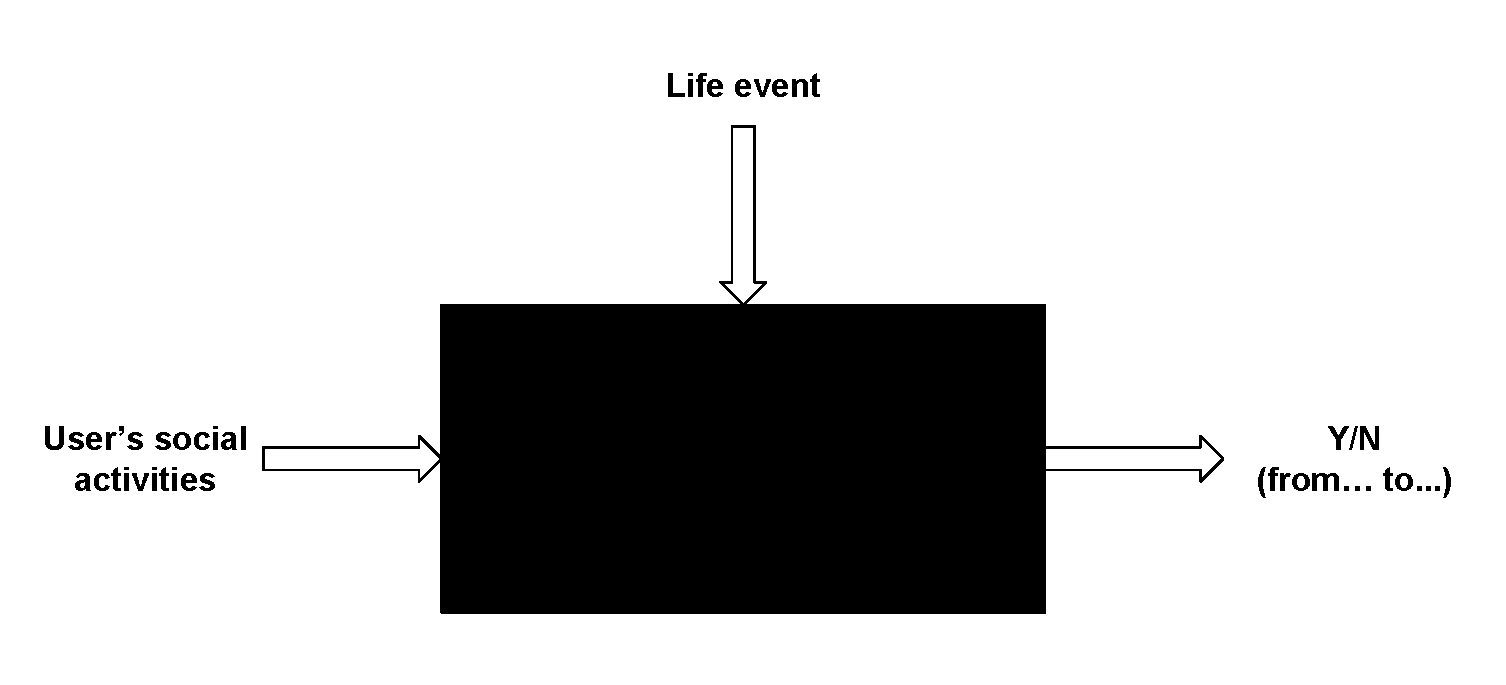
\includegraphics[width=%
0.8\textwidth]{img/bb}
\caption{A black box view of the problem.}
\label{fig:bb}
\end{figure}

The goal of this thesis is to design and develop a model that detects and predicts the occurrence of life events based on social media user activities. Seen as a blackbox like in figure~\ref{fig:bb}, it takes as input all the user's activities in the social networks he/she is registered in, and a life event to search for, and it returns as output a yes/no answer to the question "\textit{has this user lived this life event?}", with a time reference attached.

TBC: tecniche e tecnologie utilizzate
risultati o conlcusioni


